\newpage
\section{Auswertung}
\label{sec:Auswertung}
Im Folgenden werden alle Berechnungen in Python 3.7.1, unterstützt durch das
Paket NumPy \cite{numpy}, durchgeführt. Für die Ausgleichsrechnung wird SciPy
\cite{scipy} verwendet. Die Abbildungen werden mit matplotlib \cite{matplotlib} erstellt.

\subsection{Bestimmung des vertikalen Erdmagnetfeldes}
\label{subsec:vertikal}

Es wurde im Versuch mithilfe eines Helmholtzspulenpaares ein vertikales Magnetfeld
erzeugt, das die vertikale Komponente des Erdmagnetfeldes kompensierte. Die vertikale
Komponente des Erdmagnetfeldes lässt sich daher aus den Daten des Helmholtzspulenpaares
mithilfe der Formel
\begin{equation}
    B= \mu_0 \cdot  \frac{8}{\sqrt {125}}\cdot \frac{I\cdot N}{R}
    \label{eqn:Helmholtz}
\end{equation}
berechnen. Mit den Daten aus der Versuchsanleitung \cite{Versuchsanleitung} und einem Strom von
$I_{\text{vert}}=0{,}195\,$A ergibt sich die vertikale Komponente des Erdmagnetfeldes zu
\begin{equation*}
  \SI{2.99e-5}{\tesla}\,.
\end{equation*}
Der Theoriewert hierzu liegt bei $\SI{44}{\micro\tesla}$ \cite{erde}. Der gemessene Wert
weicht hiervon um $-32{,}05\%$ ab.

\subsection{Bestimmung des horizontalen Erdmagnetfeldes und der Landé-Faktoren}
\label{subsec:horizontal}

Zunächst werden mithilfe von Gleichung \eqref{eqn:Helmholtz} aus den gemessenen Stromstärken
die horizontalen Magnetfeldstärken berechnet. Die gemessenen und die daraus berechneten Werte befinden sich
in Tabelle \ref{tab:werte}.

\begin{table}[htp]
	\begin{center}
    \caption{Messwerte und daraus berechnete Werte für die magnetische Feldstärke.}
    \label{tab:werte}
		\begin{tabular}{ccccc}
		\toprule
			{$f$/kHz} & {$I_1$/A} & {$I_2$/A} & {$B_1$/µT} & {$B_2$/µT}\\
			\midrule
			100 & 0,42 & 0,50 & 25,35 & 30,17\\
			200 & 0,58 & 0,76 & 35,00 & 45,86\\
			300 & 0,76 & 1,00 & 45,86 & 60,35\\
			400 & 0,92 & 1,26 & 55,52 & 76,04\\
			500 & 1,09 & 1,51 & 65,78 & 91,12\\
			600 & 1,26 & 1,76 & 76,04 & 106,21\\
			700 & 1,43 & 2,01 & 86,30 & 121,30\\
			800 & 1,60 & 2,21 & 96,56 & 133,37\\
			900 & 1,76 & 2,52 & 106,21 & 152,08\\
			1000 & 1,93 & 2,77 & 116,47 & 167,16\\
		\bottomrule
		\end{tabular}
	\end{center}
\end{table}

Anschließend wird für beide Isotope getrennt jeweils die horizontale Magnetfeldstärke $B_{\text{hor}}$
gegen die Frequenz $f$ aufgetragen und es wird eine lineare Ausgleichsrechnung der Form
\begin{equation*}
  g(f)=af+b
\end{equation*}
durchgeführt. Es ergeben sich die Parameter
\begin{align*}
 a_1&= \SI{1.0149(0027)e-10}{\tesla\per\Hz}  \,,\\
 b_1&= \SI{1.509(016)e-05}{\tesla} \,,\\
 a_2&= \SI{1.511(012)e-10}{\tesla\per\Hz} \,,\\
 b_2&= \SI{1.53(07)e-05}{\tesla} \,.
\end{align*}
Die zugehörigen Plots sind in den Abbildungen \ref{fig:frequenz1} und \ref{fig:frequenz2} dargestellt.
Es ist erkennbar, dass die Messwerte sich sehr gut durch eine Gerade anpassen lassen.
\begin{figure}
  \centering
  \includegraphics[width=\textwidth]{build/frequenz1.pdf}
  \caption{Messwerte und Ausgleichsrechnung zur Bestimmung des horizontalen B-Feldes und des Landé-Faktors für
  das erste Isotop.}
  \label{fig:frequenz1}
\end{figure}
\begin{figure}
  \centering
  \includegraphics[width=\textwidth]{build/frequenz2.pdf}
  \caption{Messwerte und Ausgleichsrechnung zur Bestimmung des horizontalen B-Feldes und des Landé-Faktors für
  das zweite Isotop.}
  \label{fig:frequenz2}
\end{figure}

Aus den Parametern lassen sich nun die horizontale B-Feldstärke, sowie der Landé-Faktor bestimmen.
Die horizontale Erdmagnetfeldstärke ist gegeben durch den Parameter $b$. Der Theoriewert beträgt hier
$\SI{20}{\micro\tesla}$ \cite{erde}. Die Abweichung vom Theoriewert beträgt damit $-24{,}55\%$ für
$b_1$ und $-23{,}5\%$ für $b_2$.

Der Landé-Faktor kann mithilfe von Gleichung \eqref{eqn:B_M_Theorie} berechnet werden zu
\begin{equation*}
  g_F=\frac{4\pi m_e}{e a} \,.
\end{equation*}
Damit ergeben sich die beiden Werte
\begin{align*}
  g_{F,1}&= \SI{0.7041(0018)}{}\,,\\
  g_{F,2}&= \SI{0.473(004)}{}\,.
\end{align*}
Die Unsicherheiten der $g_{F,i}$ lässt sich durch
\begin{equation}
  \sigma_{g_{F,i}} = \frac{4\pi m_e}{e a_i^2} \sigma_{a_i}
  \label{eqn:sigma_g_F}
\end{equation}
bestimmen \footnote{Ist $f$ eine Funktion, die von unsicheren Variablen $x_i$ mit
Standardabweichungen $\sigma_i$ abhängt, so ist die Unsicherheit von f
\begin{equation}
  \sigma_f = \sqrt{
    \sum\limits_{i = 1}^N
      \left( \frac{\partial f}{\partial x_i} \sigma_i \right)^{\!\! 2}
  }\,.
  \label{eqn:gaussfehler}
\end{equation}
Diese Formel wird auch "Gauß'sches Fehlerfortpflanzungsgesetz" gennant.}.

\subsection{Bestimmung des Kernspins}
\label{subsec:Kernspin}

Für die beiden Rb Isotope gilt $L=0$, $S=\frac{1}{2}$ und $J=\frac{1}{2}$.
Es folgt für Gleichung \eqref{eqn:g_F_Theorie}
\begin{equation*}
  I=\frac{1}{2}\left(\frac{g_J}{g_F}-1\right) \,.
\end{equation*}
Der Landé-Faktor $g_J$ kann mithilfe von Gleichung \eqref{eqn:g_J_Theorie} zu $g_J=2{,}0023$ bestimmt
werden. Für den Kernspin folgt damit
\begin{align*}
  I_1&= \SI{0.922(004)}{}\,,\\
  I_2&= \SI{1.616(017)}{}\,.
\end{align*}
Die Theoriewerte betragen hier $I=5/2$ für $\text{Rb}^{85}$ und $I=3/2$ für $\text{Rb}^{87}$.
Die Unsicherheiten der $I_i$ sind
\begin{equation}
  \sigma_{I_i} = \frac{g_J}{2 g_{F_i}^2} \sigma_{g_{F,i}}\,.
\end{equation}
%mit $\sigma_{g_{F,i}}$ aus Gleichung \eqref{eqn:sigma_g_F}.

Mithilfe des Kernspins können die Isotope wie folgt zugeordnet werden: Isotop 1 ist $\text{Rb}^{87}$
und Isotop 2 ist $\text{Rb}^{85}$. Die Abweichungen von den Theoriewerten betragen
$-35{,}36\%$ für $\text{Rb}^{85}$ und $-38{,}53\%$ für $\text{Rb}^{87}$.


\subsection{Bestimmung des Isotopenverhältnisses}
\label{subsec:Isotope}
In Abbildung \ref{fig:foto} ist ein typischer Verlauf der Transparenz des Rb-Gases in Abhängigkeit
von der magnetischen Feldstärke bei einer Frequenz von $f=100\,$kHz dargestellt.
Aus dem Verhältnis der Tiefen der Dips der beiden
Isotope lässt sich mithilfe von Gleichung \eqref{eqn:transient} das Isotopenverhältnis bestimmen.
Für den ersten Dip ergibt sich eine Amplitude von 4{,}5 Einheiten und für den zweiten
eine Amplitude von 9 Einheiten
\begin{equation*}
  \frac{\gamma_{85}}{\gamma_{87}}=\frac{9}{4{,}5}= 2 \,.
\end{equation*}

Das in der Natur vorkommende Verhältnis folgt aus den Verhältnissen der beiden Isotope \cite{verhältnis}
und ergibt
\begin{equation*}
  \frac{\text{Anteil}~ \ce{^{85}Rb}}{\text{Anteil}~ \ce{^{87}Rb}}=\frac{72,17\%}{27,83\%} \approx 2{,}593 \,.
\end{equation*}
Der aus den Messwerten berechnete Wert weicht davon um $-22{,}87\%$ ab.

\begin{figure}
  \centering
  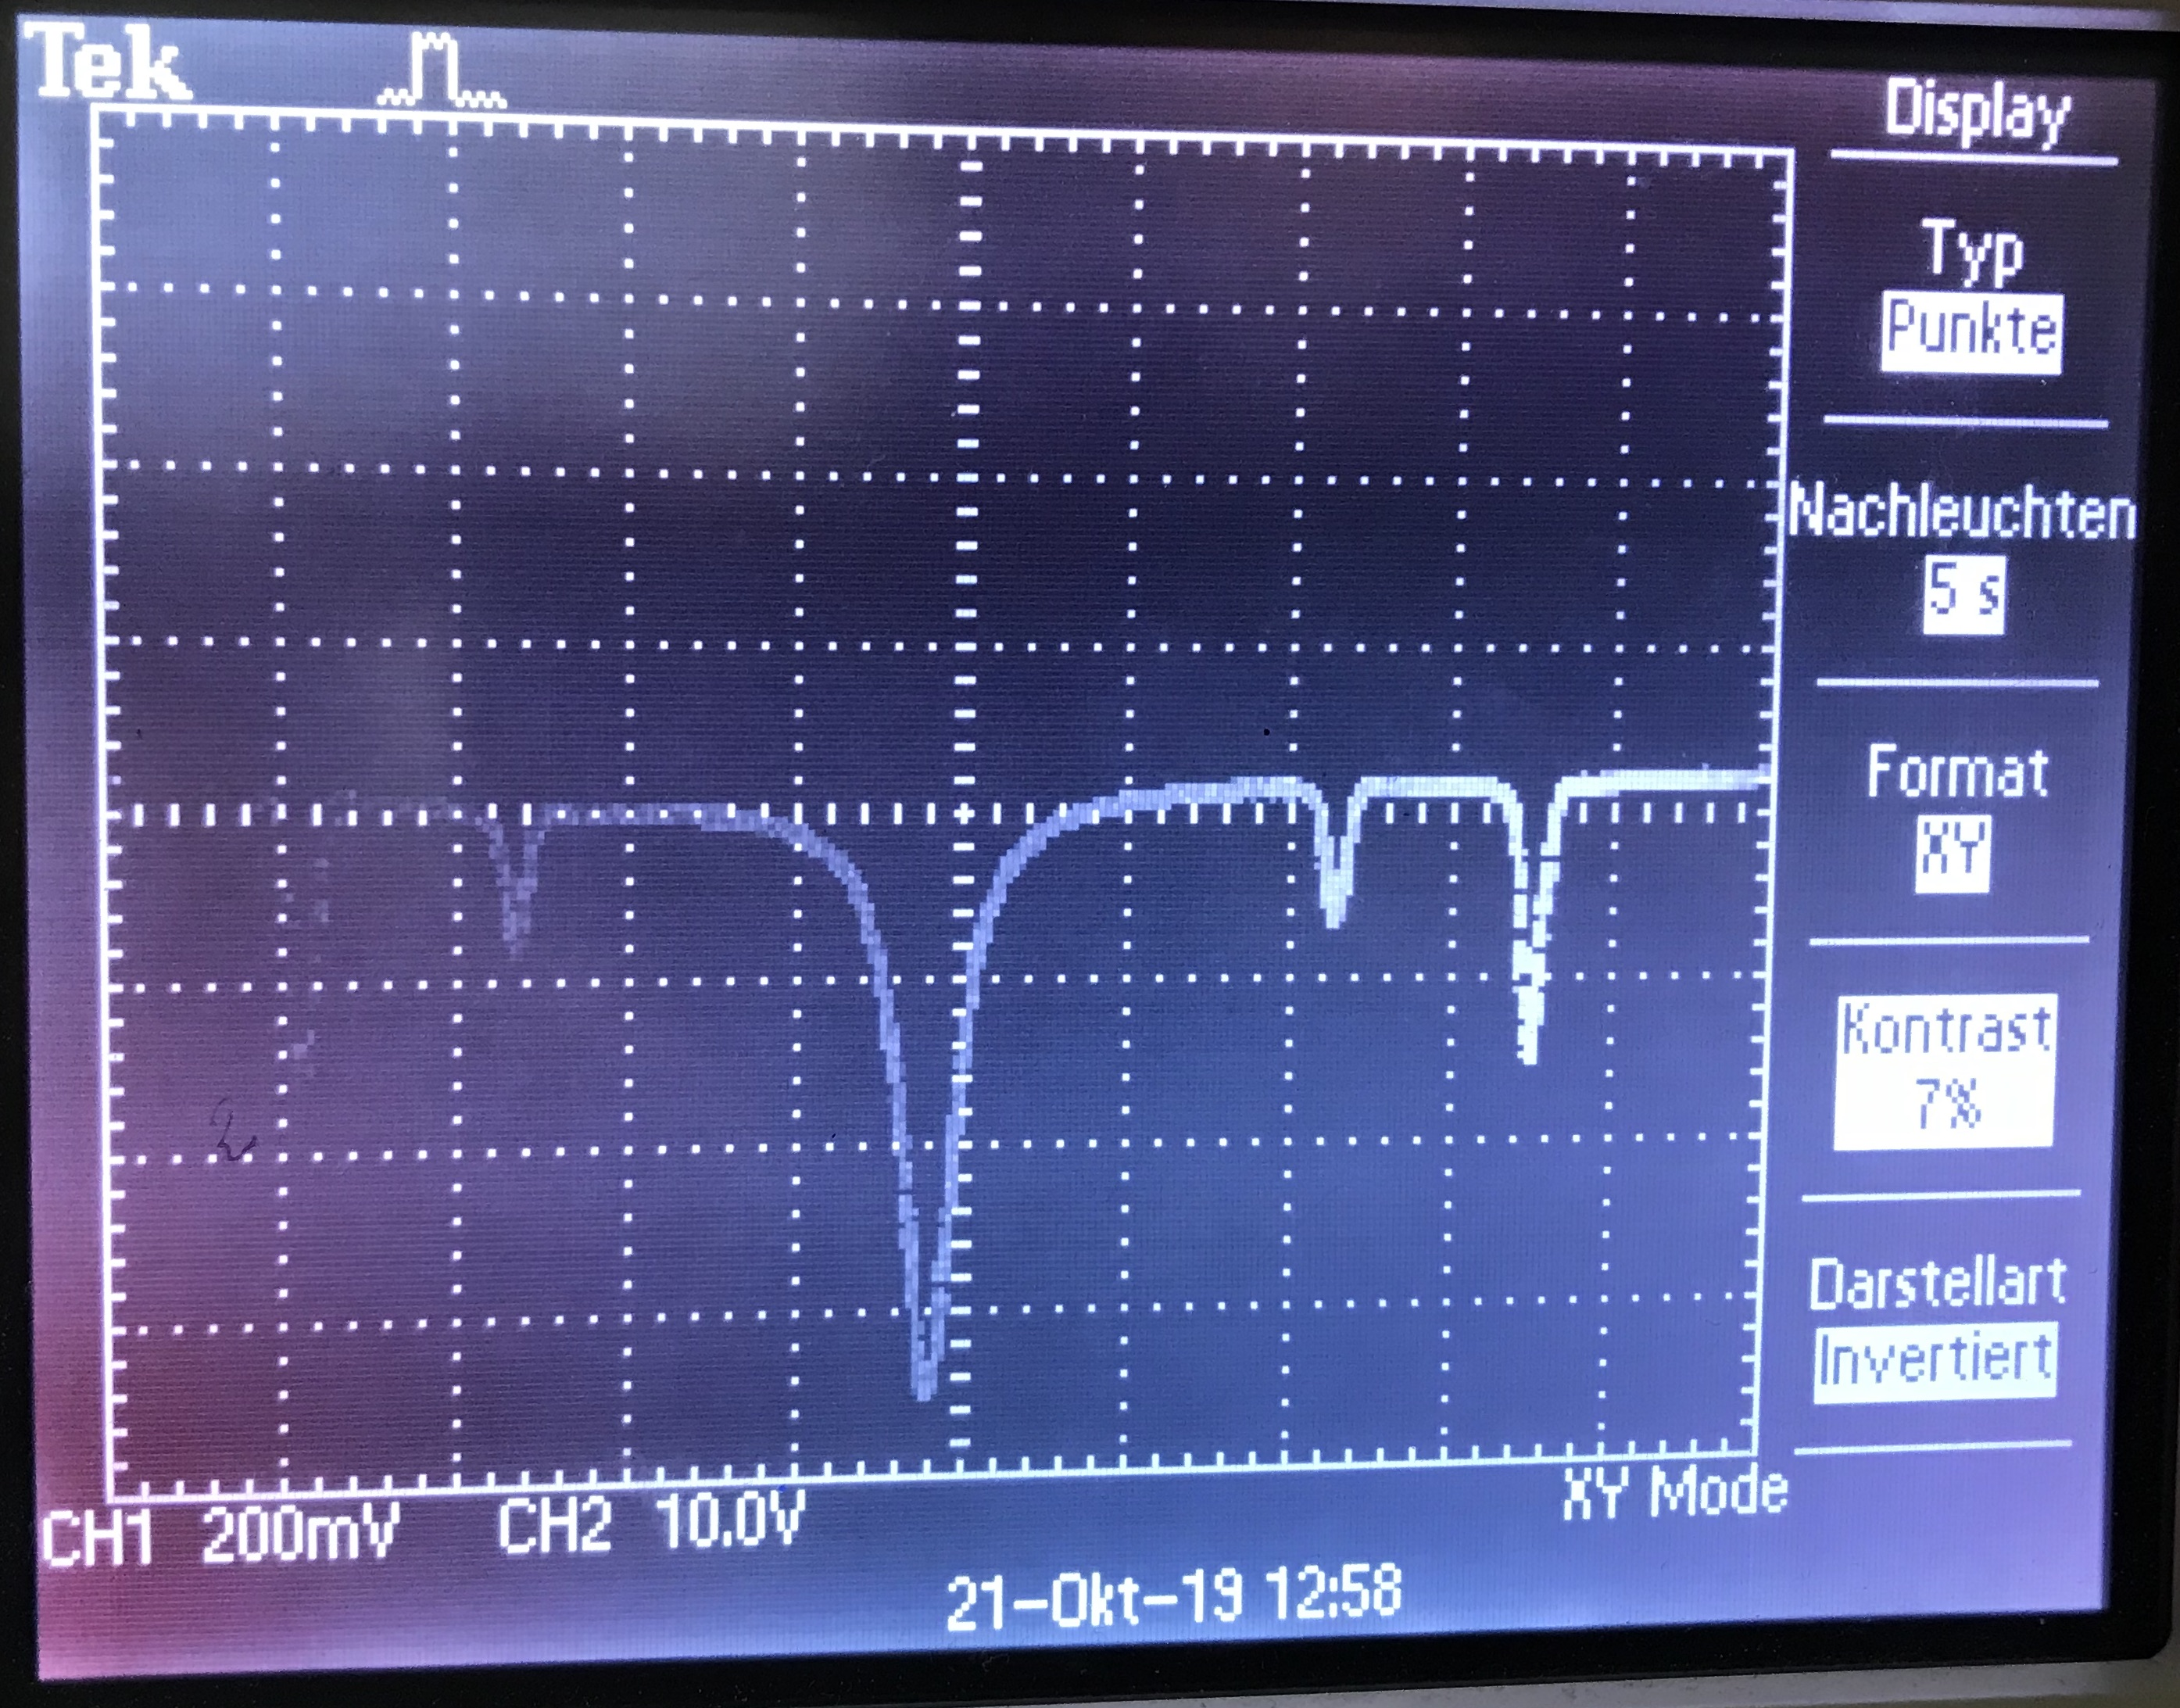
\includegraphics[width=0.7\textwidth]{data/foto.jpg}
  \caption{Typischer Verlauf der Transparenz des Rb-Gases in Abhängigkeit von der magnetischen Feldstärke bei einer Frequenz von $f=100\,$kHz.}
  \label{fig:foto}
\end{figure}


\subsection{Abschätzung des quadratischen Zeeman-Effekts}
\label{subsec:zeeman}
In diesem Kapitel soll abgeschätzt werden, wie groß der Einfluss des quadratischen Zeeman-Effekts
in diesem Versuch ist. Der quadratische Zeeman-Effekt kann durch Gleichung
\eqref{eqn:zeemanDifferenzQuadratisch} beschrieben werden. Gemäß der Versuchsanleitung \cite{Versuchsanleitung} beträgt die
Hyperfeinstrukturaufspaltung des Grundzustandes
\begin{align*}
  \Delta E_{85}&= \SI{2.01e-24}{\joule}\,,\\
  \Delta E_{87}&= \SI{4.53e-24}{\joule}\,.
\end{align*}
Mit den jeweiligen berechneten Werten $B_i$ für die Horizontalkomponente des Erdmagnetfeldes,
$g_{F,i}$ für die Landé-Faktoren und $M_F=1$ ergibt sich damit für den quadratischen Zeeman-Effekt
\begin{align*}
  \Delta E_{Z,85}&=\SI{6.7(4)e-29}{\joule}\,,\\
  \Delta E_{Z,87}&=\SI{9.85(13)e-29}{\joule}\,.
\end{align*}
Die Unsicherheiten der $\Delta E_{Z,i}$ betragen
\begin{equation}
  \sigma_{\Delta E_{Z,i}} = \left( \mu_{\text{B}} B + 2 g_{F,i} \mu_{\text{B}}^2 B^2 \frac{1 - 2 M_F}{\Delta E_{\text{Hy}}} \right) \sigma_{g_{F,i}}\,.
  \label{eqn:sigma_Delta_E_Z}
\end{equation}

Die zusätzlich zum linearen Zeeman-Effekt durch den quadratischen Term herbeigeführte Aufspaltung beträgt dabei lediglich
\begin{align*}
  \Delta E_{\text{quadratisch},85}&=\SI{-2.24(25)e-33}{\joule}\,,\\
  \Delta E_{\text{quadratisch},87}&=\SI{-2.14(06)e-33}{\joule}\,,
\end{align*}
wobei die Unsicherheiten durch den zweiten Term in Gleichung \eqref{eqn:sigma_Delta_E_Z} beschrieben werden.
Somit ist der quadratische Zeeman-Effekt in diesem Versuch vernachlässigbar.

\subsection{Anpassung der ansteigenden Flanken an eine Exponentialfunktion}
\label{subsec:flanken}

In diesem Kapitel sollen die ansteigenden Flanken aus dem letzten Versuchsteil an
Exponentialfunktionen angepasst werden. Dafür werden zunächst Werte aus den angefertigten
Bildern abgelesen. Die Aufnahmen des Oszilloskops befinden sich in den Abbildungen
\ref{fig:flanke1} und \ref{fig:flanke2}. Die daraus abgelesenen Werte befinden sich in
Tabelle \ref{tab:flanke}.

\begin{figure}
  \centering
  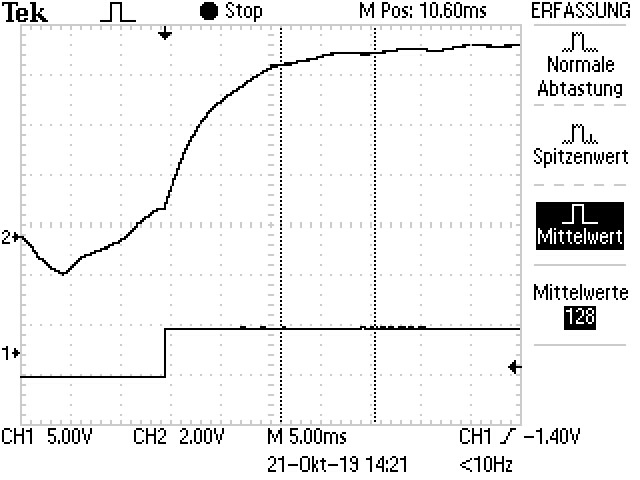
\includegraphics[width=0.7\textwidth]{data/Dip1.jpg}
  \caption{Ansteigende Flanke für den ersten Dip.}
  \label{fig:flanke1}
\end{figure}
\begin{figure}
  \centering
  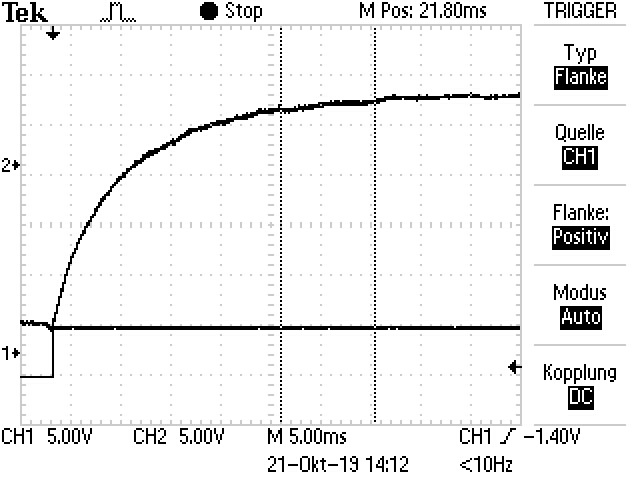
\includegraphics[width=0.7\textwidth]{data/Dip2.jpg}
  \caption{Ansteigende Flanke für den zweiten Dip.}
  \label{fig:flanke2}
\end{figure}

\begin{table}[htp]
	\begin{center}
    \caption{Aus den Bildern abgelesene und auf 1 normierte Werte für die Transparenz in Abhängigkeit von der Zeit.}
    \label{tab:flanke}
		\begin{tabular}{cccc}
		\toprule
			{$t_1$/ms} & {$\text{Transparenz}_1$} & {$t_2$/ms} & {$\text{Transparenz}_2$}\\
			\midrule
			22,5 & 0,09 & 15,0 & 0,00\\
			25,0 & 0,23 & 20,0 & 0,18\\
			30,0 & 0,34 & 25,0 & 0,29\\
			35,0 & 0,51 & 30,0 & 0,40\\
			40,0 & 0,57 & 35,0 & 0,49\\
			45,0 & 0,66 & 40,0 & 0,56\\
			50,0 & 0,69 & 45,0 & 0,62\\
			55,0 & 0,74 & 50,0 & 0,67\\
			60,0 & 0,77 & 55,0 & 0,71\\
			65,0 & 0,80 & 60,0 & 0,73\\
			70,0 & 0,86 & 65,0 & 0,76\\
			75,0 & 0,91 & 70,0 & 0,78\\
			80,0 & 0,91 & 75,0 & 0,80\\
			85,0 & 0,94 & 80,0 & 0,82\\
			90,0 & 0,94 & 85,0 & 0,84\\
			95,0 & 0,97 & 90,0 & 0,87\\
			100 & 0,97 & 95,0 & 0,89\\
			105 & 0,97 & 100 & 0,91\\
			110 & 0,97 & 105 & 0,91\\
			115 & 0,97 & 110 & 0,93\\
			120 & 0,97 & 115 & 0,93\\
			125 & 0,97 & 120 & 0,96\\
			130 & 0,97 & 125 & 0,96\\
			135 & 1,00 & 130 & 0,96\\
			140 & 1,00 & 135 & 0,96\\
			145 & 1,00 & 140 & 0,98\\
			150 & 1,00 & 145 & 0,98\\
			- & - & 150 & 0,98\\
			- & - & 155 & 1,00\\
			- & - & 160 & 1,00\\
			- & - & 165 & 1,00\\
			- & - & 170 & 1,00\\
			- & - & 175 & 1,00\\
			- & - & 180 & 1,00\\
			- & - & 185 & 1,00\\
			- & - & 190 & 1,00\\
		\bottomrule
		\end{tabular}
	\end{center}
\end{table}

Die Werte werden auf 1 normiert. Anschließend wird eine Ausgleichsrechnung der Form
\begin{equation*}
  f(t)=1-\exp(-a(t-b))
\end{equation*}
durchgeführt. Es ergeben sich die Parameter
\begin{align*}
  a_1&=\SI{0.0398(0010)}{\per\milli\second} \,,\\
  b_1&=\SI{19.2(4)}{\milli\second} \,,\\
  a_2&=\SI{0.0285(0005)}{\per\milli\second}\,,\\
  b_2&=\SI{13.3(5)}{\milli\second} \,.
\end{align*}
In den Abbildungen \ref{fig:flankefit1} und \ref{fig:flankefit2} sind die Messwerte und die
Ausgleichsrechnungen grafisch dargestellt. Es ist erkennbar, dass sich die Messwerte gut
durch eine Exponentialfunktion annähern lassen.

\begin{figure}
  \centering
  \includegraphics[width=\textwidth]{build/flanke1.pdf}
  \caption{Messwerte und Ausgleichsfunktion für den ersten Dip.}
  \label{fig:flankefit1}
\end{figure}
\begin{figure}
  \centering
  \includegraphics[width=\textwidth]{build/flanke2.pdf}
  \caption{Messwerte und Ausgleichsfunktion für den zweiten Dip.}
  \label{fig:flankefit2}
\end{figure}

\newpage
\subsection{Bestimmung des Verhältnisses der Landé-Faktoren mithilfe der Rabi-Oszillationen}
\label{subsec:oszillationen}
Zur Bestimmung des Verhältnisses der Landé-Faktoren mithilfe der Rabi-Oszillationen werden
die gemessenen Periodendauern der Oszillationen gegen die Amplitude des RF-Feldes aufgetragen.
Die zugehörigen Messwerte befinden sich in Tabelle \ref{tab:oszi}.

\begin{table}[htp]
	\begin{center}
    \caption{Messwerte für die Periodendauern der Oszillationen in Abhängigkeit von der Amplitude des RF-Feldes.}
    \label{tab:oszi}
		\begin{tabular}{ccc}
		\toprule
			{$U$/V} & {$T_1$/ms} & {$T_2$/ms}\\
			\midrule
			2 & 1,50 & 2,52\\
			3 & 1,16 & 1,84\\
			4 & 0,89 & 1,29\\
			5 & 0,71 & 1,07\\
			6 & 0,61 & 0,90\\
			7 & 0,51 & 0,77\\
			8 & 0,45 & 0,67\\
			9 & 0,40 & 0,60\\
			10& 0,36 & 0,54\\
		\bottomrule
		\end{tabular}
	\end{center}
\end{table}

Außerdem wird eine Ausgleichsrechnung der Form
\begin{equation*}
  f(x)=a+\frac{b}{x-c}
\end{equation*}
durchgeführt. Dies ist in den Abbildungen \ref{fig:oszi1} und \ref{fig:oszi2} grafisch dargestellt.
Es ergeben sich die Parameter
\begin{align*}
  a_1&=\SI{-0.14(4)e-3}{\second} \,,\\
  b_1&=\SI{5.5(5)e-3}{\volt} \,,\\
  c_1&=\SI{-1.34(24)}{\volt} \,,\\
  a_2&=\SI{-7(8)e-05}{\second} \,,\\
  b_2&=\SI{6.2(7)e-3}{\volt} \,,\\
  c_2&=\SI{-0.39(22)}{\volt} \,.
\end{align*}
Das Verhältnis der Parameter $b_i$ für $\text{Rb}^{85}$ und $\text{Rb}^{87}$ beträgt damit:
\begin{equation*}
  \frac{b_2}{b_1}\approx\SI{1.13(17)}{}\,
\end{equation*}
mit der Unsicherheit
\begin{equation}
  \sigma_{b_2/b_1} = \sqrt{\left( \frac{1}{b_1}\sigma_{b_2} \right)^2 + \left( \frac{b_2}{b_1^2} \sigma_{b_1} \right)^2}
\end{equation}
Dieser Wert weicht um $-24{,}67\%$ vom Theoriewert 1{,}5 ab.
\begin{figure}
  \centering
  \includegraphics[width=\textwidth]{build/oszi1.pdf}
  \caption{Messwerte und Ausgleichsrechnung zur Bestimmung des Verhältnisses der Landé-Faktoren mithilfe der
  Rabi-Oszillationen für $\text{Rb}^{87}$.}
  \label{fig:oszi1}
\end{figure}
\begin{figure}
  \centering
  \includegraphics[width=\textwidth]{build/oszi2.pdf}
  \caption{Messwerte und Ausgleichsrechnung zur Bestimmung des Verhältnisses der Landé-Faktoren mithilfe der
  Rabi-Oszillationen für $\text{Rb}^{85}$.}
  \label{fig:oszi2}
\end{figure}
